\RequirePackage{fixltx2e} %This package in CTeX is not compatible with revtex4-1
\documentclass[aps,pre,12pt,preprint,onecolumn,showpacs,showkeys]{revtex4-1}
\usepackage{ctex}
\usepackage{mathtools,mathrsfs}
\usepackage{multirow}
\usepackage{setspace,dcolumn}
\usepackage{hyperref}
\usepackage{graphicx,psfrag,epsfig}
\usepackage[font=small,format=plain,labelfont=bf,textfont=it,justification=centering,singlelinecheck=false]{caption}
\usepackage{amsmath,amsfonts,amssymb,amsthm,bm,upgreek}
\usepackage{geometry}
\usepackage[mathscr]{eucal}
\usepackage{caption}
\usepackage{subcaption}
\hypersetup{colorlinks=true}
\geometry{top=2.54cm,bottom=2.54cm,left=3cm,right=3cm}
\renewcommand\appendixname{附录}
\renewcommand\abstractname{}%摘要
\renewcommand\tablename{表}
\renewcommand\figurename{图}
\makeatletter
\def\@pacs@name{\songti\zihao{-4}{\bf PACS码:}}
\def\@keys@name{\songti\zihao{-4}{\bf 关键词:}}
\def\Dated@name{日期:}
\def\Received@name{\zihao{-5}{接收} }
\def\Revised@name{\zihao{-5}{修订} }
\def\Accepted@name{\zihao{-5}{采纳} }
\def\Published@name{\zihao{-5}{发表} }
\makeatother
\linespread{1.3}
\renewcommand{\labelenumi}{\alph{enumi}.}
\leftmargini=20mm
\def \d {\mathrm d}
\def \degree {^\circ}
\def \V {\bm{V}}
\def \degC {^\circ \mathrm{C}}

\begin{document}
\title{\bf\heiti\zihao{3}用$\beta$粒子验证相对论的动量-动能关系\vspace{15mm}}
\author{\fangsong\zihao{4}邵智轩\vspace{2mm}}
\affiliation{\songti\zihao{-4}学号:1400012141\vspace{2mm}}
\date{\today}
%\pacs{02.10.Yn, 33.15.Vb, 98.52.Cf, 78.47.dc}
\keywords{狭义相对论,$\beta$衰变,$\beta$磁谱仪,闪烁体探测器}
\email{shaozhixuansh@pku.edu.cn; (86)13381350619}

\begin{abstract}
\vspace{10mm}
\begin{spacing}{1.5}
\songti\zihao{-4}
本实验通过同时测量速度接近光速$c$的高速电子的动量和动能,来验证狭义相对论中动能与动量关系的正确性,并学习$\beta$磁谱仪的测量原理及其他核物理的实验方法和技术。

\end{spacing}
\end{abstract}
\maketitle
\songti\zihao{-4}

\section{引言}
    狭义相对论已为大量的实验所证实,并应用于近代物理的各个领域。本实验通过同时测量速度接近光速$c$的高速电子的动量和动能,来证明狭义相对论的正确性,并学习$\beta$磁谱仪的测量原理及其他核物理的实验方法和技术。

\section{实验原理}
    \subsection{相对论动量-动能关系}
    四-动量$\bm{P}$可写成
    \begin{equation}
        \bm{P}=(p^0, p^1, p^2, p^3)=(\frac{E}{c}, \bm{p}),
    \end{equation}
    其中三-动量$\bm p=\gamma m_0 \bm v =\gamma m_0 (v_1, v_2, v_3)$,$E=\gamma m_0 c^2$。四-动量$\bm P$的Minkowski内积是Lorentz不变量:
    \begin{equation}
        -(\frac{E}{c})^2+p^2=-(\frac{E'}{c})^2+p'^2,\label{eq:invariant}
    \end{equation}
    其中$p^2=|\bm p|^2=p_1^2+p_2^2+p_3^2$。若取$S'$为于物体静止的参考系,有$\bm {p'}=\bm{0}$,$E'=E_0=m_0 c^2$,则(\ref{eq:invariant})写为:
    \begin{equation}
        E^2-c^2 p^2 =E_0^2
    \end{equation}
    这就是相对论的能量和动量关系,而动能和动量的关系为:
    \begin{equation}
        E_k=E-E_0=(c^2p^2+m_0 ^2 c^4)^{1/2}-m_0 c^2\label{eq:relationship}
    \end{equation}

    \subsection{$\beta$磁谱仪与动量测量}
    高速$\beta$粒子在垂直于运动方向的均匀磁场$B$中的运动方程为
    \begin{equation}
        m\frac{v^2}{R}=\frac{\d p}{\d t}=evB
    \end{equation}
    从而
    \begin{equation}
        p=eBR
    \end{equation}
    $R$为$\beta$粒子轨道半径,是源与探测器间距的一半。移动探测器即改变$R$,可得到不同动量的$\beta$粒子。

\section{实验内容}
    \subsection{闪烁计数器能量定标}
    $\beta$粒子的动能$E_i$与多道分析器的道数$n$成正比:
    \begin{equation}
        E_i=a+bn
    \end{equation}
    \begin{figure}[ht]
        \centering
        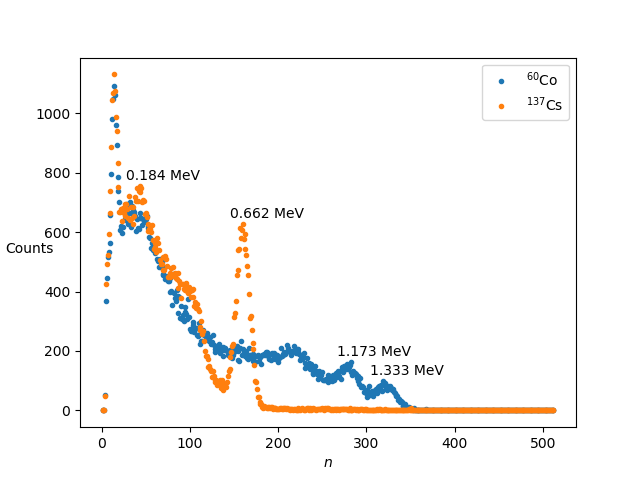
\includegraphics[width=120mm]{Co60_Cs137}
        \caption{\label{fig:Co60_Cs137}%
        $^{60}$Co 和$^{137}$Cs 的计数-道数关系曲线}
    \end{figure}
    可用几个已知能量的放射源来标定待定参数$a$和$b$,常用的标准源有$^{137}$Cs $\gamma$射线的0.662 MeV的光电峰和0.184 MeV的反射峰;$^{60}$Co $\gamma$射线的的1.173 MeV和1.333 MeV的两个光电峰。固定光电管的高电位于594 V, 增益倍数为一固定位置,他们的计数-道数关系曲线如图\ref{fig:Co60_Cs137}所示,各峰对应的道数如表\ref{tab:Co60_Cs137}所示。


    \begin{table}[h]
        \caption{\label{tab:Co60_Cs137}%
        用$^{60}$Co 和$^{137}$Cs 放射源进行能量定标}
        \begin{tabular}{|c|c|c|c|c|}
            \hline
            & $^{137}$Cs 反散射峰 & $^{137}$Cs 光电峰 & $^{60}$Co 光电峰1 & $^{60}$Co 光电峰2\\\hline
        $E_i$/MeV & 0.184 & 0.662 & 1.173 & 1.333\\\hline
        道数 $n$ & 43 & 160 & 282 & 319 \\\hline
        \end{tabular}
    \end{table}
    拟合直线的相关系数$r=0.99996$,回归系数为:
    \begin{equation}
        a=1.7027 \times 10 ^{-3}, \quad b=4.1607 \times 10 ^{-3} 
    \end{equation}

    \subsection{测量不同动量的$\beta$粒子的相应动能}
    保持光电管的电压与放大倍数不变。$\beta$粒子放射源置于位置刻度线的$6.00$ cm 处,粒子进入均匀磁场下的真空室,均匀磁场大小为$B=0.06555$ T。将闪烁体探测器探头置于不同位置$x$处(在真空室的每一个窗口取一点),分别测定对应的$\beta$能谱的峰位,并记录探头的位置,记录的数据如表\ref{tab:beta}所示。

    \begin{table}[h]
        \caption{\label{tab:beta}%
        测量不同动量的$\beta$粒子的相应动能(真空)}
        \begin{tabular}{|c|c|c|c|c|c|c|}
            \hline
            $x$/cm & 28.55 & 25.70 & 23.60 & 21.10 & 18.55 & 16.25\\\hline 
            $R$/cm\footnote{$R=\frac{1}{2}(x-6.15)$} & 11.20 & 9.78 & 8.73 & 7.48 & 6.20 & 5.05\\\hline
            $pc$/MeV \footnote{$pc/\mathrm{MeV}=3(B/\mathrm{T})(R/\mathrm{cm})$}& 2.201 & 1.922 & 1.715 & 1.469 & 1.218 & 0.992\\\hline
            道数$n$ & 398 & 333 & 276 & 223 & 166 & 109 \\\hline
            $E_t$/MeV\footnote{$E_t=a+bn$} & 1.658 & 1.387 & 1.150 & 0.930 & 0.692 & 0.455 \\\hline
            $E_i$/MeV & 1.747 & 1.475 & 1.239 & 1.018 & 0.782 & 0.550 \\\hline
        \end{tabular}
    \end{table}

    狭义相对论理论下,动能和动量的关系为\ref{eq:relationship},代入电子的静能$m_0 c^2 = 0.511$ MeV,以 MeV 为单位,有
    \begin{equation}
        E_k = \sqrt{(cp)^2 +0.511 ^2}-0.511
    \end{equation}
    而经典理论(伽利略时空观)下的动能动量关系为:
    \begin{equation}
        E_k =\frac{ (cp)^2 }{2 \times 0.511}
    \end{equation}
    \begin{figure}[ht]
        \centering
        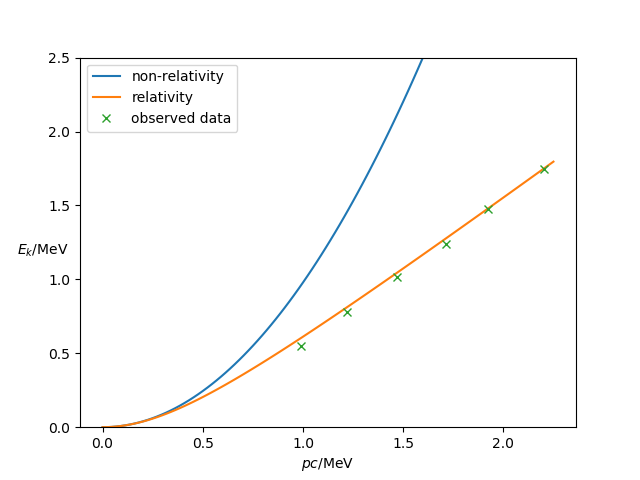
\includegraphics[width=120mm]{relationship}
        \caption{\label{fig:relationship}%
        经典力学与狭义相对论的动能-动量关系,以及实测$\beta$粒子的动能-动量关系}
    \end{figure}
    它们在高能端有显著的差异,如图\ref{fig:relationship}所示。我们将表\ref{tab:beta}中的6个数据点也标在图中。可以看到,相对论动量-动能关系与实验相符。

    此外还在大气中重复了以上实验,数据如表\ref{tab:beta_atmo}所示。
    \begin{table}[h]
        \caption{\label{tab:beta_atmo}%
        测量不同动量的$\beta$粒子的相应动能(大气)}
        \begin{tabular}{|c|c|c|c|c|}
            \hline
            $x$/cm & 16.25 & 21.10 & 25.70\\\hline 
            $R$/cm & 5.05 & 7.48 & 9.78\\\hline
            $pc$/MeV & 0.992 & 1.469 & 1.922\\\hline
            道数$n$ & 108 & 214 & 324\\\hline
            $E_t$/MeV &0.451 & 0.892 & 1.350 \\\hline
            $E_i$/MeV &0.546 & 0.980 & 1.435\\\hline
        \end{tabular}
    \end{table}
    对比真空中的结果,不同之处有两点:其一,峰的半高宽变宽;其二,峰位对应的能量偏小,且越往高能端越明显。这是由于真空度降低、压强升高后,电子的平均自由程减小,与空气分子的碰撞增多,使得两侧轨道的相近能量的电子更多地散射至探测器所在轨道,使展宽变宽;而从统计意义上说,内侧轨道的低能电子散射至探测器的概率更大,使峰位对应的能量略有降低。

\section{结论}
本实验通过同时测量速度接近光速$c$的高速电子的动量和动能,定量地验证了狭义相对论中动量-动能关系(\ref{eq:relationship})的正确性,并学习$\beta$磁谱仪的测量原理及其他核物理的实验方法和技术。

\section{致谢}
感谢张双全老师对实验的悉心指导,使我掌握了$\beta$磁谱仪的使用方法。张老师主张让我们自己多琢磨试错,勤于思考,这种精神让我受益匪浅。
    
\begin{thebibliography}{}
\bibitem{Book} 吴思诚, 荀坤. 近代物理实验(第四版). 北京:高等教育出版社, 2015
\end{thebibliography}
\end{document}